\apendice{Documentación técnica de programación}

\section{Introducción}
En este anexo se introducirá todos los directorios, \textit{notebooks} y documentación útil necesaria para las personas que deseen continuar o trabajar en el proyecto.

\section{Estructura de directorios}
La estructura de directorios del proyecto, en estructura de árbol, es la siguiente:

\begin{itemize}
	\item \textit{\textbf{/}}, es decir, el directorio raíz. En el se encuentra el fichero de la licencia, el \textit{README}, el \textit{.gitignore} y las siguientes carpetas:
	\begin{itemize}
		\item \textit{\textbf{code}}: contiene toda la lógica de la aplicación.
			\begin{itemize}
				\item \textit{\textbf{imgaug}}: repositorio para realizar \textit{Data Augmentation} con \textit{Python 2}.
				\item \textit{\textbf{darkflow}}: repositorio para la detección de objetos en tiempo real.
				\item \textit{\textbf{notebooks}}: contiene todos los notebooks creados para este proyecto.
				\begin{itemize}
					\item Classifiers\_and\_HoG: contiene una serie de \textit{notebooks} para la clasificación de imágenes.
					\item Data\_Augmentation: contiene una serie de \textit{notebooks} para tareas de \textit{data augmentation}.
					\item Image\_Labeler: contiene el etiquetador de imágenes.
					\item Phytoliths\_Classifier: contiene varios \textit{notebooks} en los que se muestran ejemplos de clasificación y reconocimiento de fitolitos.
					\item Prototypes: contiene varios \textit{notebooks} prototipos.
				\end{itemize}
				\item \textit{\textbf{rsc}}: contiene los recursos necesarios por las distintas aplicaciones: imágenes y objetos. 
			\end{itemize}
		\item \textit{\textbf{doc}}: contiene la documentación del proyecto.
		\begin{itemize}
			\item \textbf{general\_doc}: contiene la memoria y los anexos del proyecto.
				\begin{itemize}
					\item \textit{\textbf{img}}: contiene todas las imágenes de la memoria y anexos del proyecto.
					\item \textit{\textbf{tex}}: contiene los ficheros correspondientes a cada uno de los anexos.
				\end{itemize}
			\item \textbf{source\_doc}: contiene la documentación del código.
			\item \textbf{test\_reports}: contiene los informes de cubrimiento del código.
		\end{itemize}
	\end{itemize}
\end{itemize}

\section{Manual del programador}

En este apartado se explican algunos aspectos sobre los dos \textit{notebooks} principales: etiquetador de imágenes y \textit{notebook} para el reconocimiento de fitolitos. Aunque sería aplicable a otros, como los desarrollados para realizar \textit{data augmentation}. 

\subsection{Etiquetador de imágenes}

En esta sección explicare más en detalle como funciona internamente el etiquetador.

\subsubsection{Base del etiquetador: \textit{Widgets} de \textit{ipywidgets}}

El etiquetador está creado mediante los \textit{Widgets} de \textit{ipywidgets} para \textit{Python}. Un \textit{Widget} es un objeto de Python con representación en navegadores. Este nos permite la comunicación entre \textit{JavaScript} y \textit{Python}. Facilitando, así, crear interfaces \textit{Web} interactivas, como es nuestro caso~\cite{ipywidgets:whataarewidgets}.

El etiquetador de imágenes es un \textit{Widget} personalizado, el cual ha sido creado por nosotros. Pero, además, este utiliza otros \textit{Widgets} prefedefinidos por los \textit{ipywidgets} para los botones.

\subsubsection{\textit{Javascript}}

La parte de código \textit{JavaScript} se ocupa de representar todos los elementos visuales y capturar los eventos.

En cuanto a elementos visuales, nos referimos al SVG, la imagen, rectangulos o etiquetas y textos. Los cuales son elementos \textit{HTML}. Y, en cuanto a eventos, nos referimos a los clicks o movimientos del ratón sobre nuestros elementos \textit{HTML}.

\subsubsection{\textit{Python}}

La parte de \textit{Python} controla toda la lógica de la aplicación. Desde que imagen se muestra, hasta las conversiones de las coordenadas de la imagen entre la vista y la imagen real.

Además, para los botones, los cuales son \textit{Widgets} de \textit{Python}, se controlan tambien sus eventos desde el propio \textit{Python}.

\subsection{Reconocimiento de fitolitos}

El \textit{notebook} para el reconocimiento de fitolitos ha sido creado basándonos en los \textit{widgets} predefinidos sobre los que en la sección anterior hablábamos. Por lo que la idea es similar a la anterior con la diferencia de que no se utiliza ningún \textit{widget} personalizado.

En cuanto al código que se encarga de detectar los fitolitos dentro de una imagen, este se encuentra documentado en la carpeta <<doc/general\_doc>> como previamente he indicado. En la figura~\ref{fig:D.3} muestro la portada de la documentación del código. Además, para tener una mayor compresión del código, se deben de consultar los anexos de diseño procedimental y los conceptos y aspectos relevantes de la memoria.

\begin{figure}
\centering
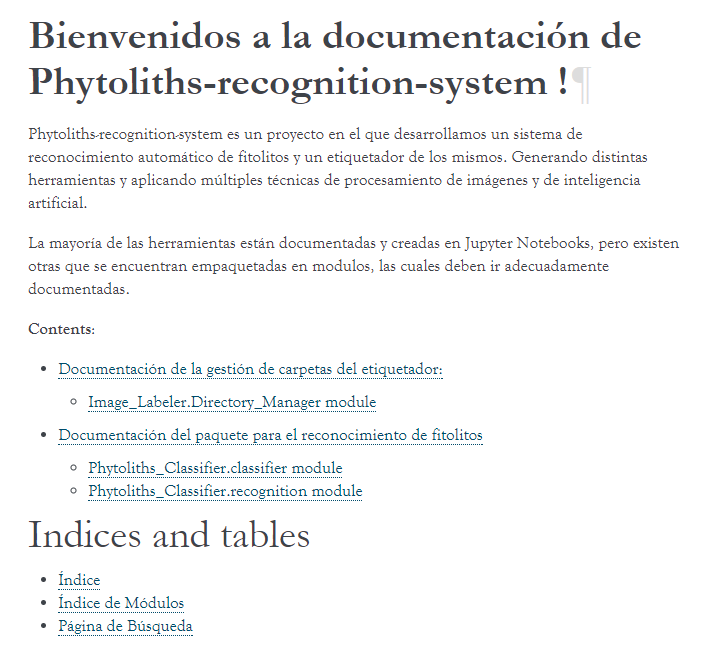
\includegraphics[width=0.99\textwidth]{docex}
\caption{Portada de la documentación del código}
\label{fig:D.3}
\end{figure}

\section{Compilación, instalación y ejecución del proyecto}

\subsection{Compilación, instalación y ejecución}

Los \textit{notebooks} llevan consigo la instalación de varias librerías, las cuales se indican en el \textit{Manual de uuario}. En ningún caso necesitan ser compilado, ni los \textit{notebooks} ni ningun fuente, al ser \textit{Python} un lenguaje interpretado.  

\subsection{Procedimiento de entrenamiento de \textit{YOLO}}

Para realizar el entrenamiento de \textit{YOLO}, \textit{darkflow} nos provee de un \textit{script} que nos facilita dicha tarea mediante la linea de comandos\footnote{Solo ha sido probado desde un sistema Linux.}, llamado \textit{flow}. Además, existen dos posibilidades principales para realizar el entrenamiento sobre nuestro \textit{dataset}:

\begin{itemize}
	\item Utilizar unos pesos\footnote{Pesos: son cada uno de los valores asignados a una neurona en una red neuronal.} pre-entrenados para nuestro modelo.
	\item Crear un modelo que se ajuste a nuestras necesidades.
\end{itemize}

La ventaja de utilizar unos pesos pre-entrenados reside en que la red neuronal ya habrá aprendido ciertas características, como bordes o formas. Por lo tanto, el tiempo de entrenamiento será mucho menor. Pero puede que la reutilización de dicho modelo no se adecue a nuestras necesidades ya sea porque tengamos un número distinto de clases al modelo inicial o porque el contexto sea totalmente distinto.

Por otro lado, se encuentra el entrenamiento desde cero de un nuevo modelo que se adecue a nuestras necesidades. El cual suple las desventajas presentadas por la anterior opción, pero introduce una mayor complejidad a la hora del entrenamiento.

En cualquier caso, los dos siguientes ejemplos, correspondientes a las opciones planteadas, nos permitirían entrenar el modelo:

\begin{verbatim}
flow --train --model cfg/yolo-tiny.cfg
 --load bin/yolo-tiny.weights
 --dataset "Fitolitos" --annotation "Fitolitos"

o

flow --model cfg/yolo-new.cfg --train
 --dataset "Fitolitos" --annotation "Fitolitos"
\end{verbatim}

Donde la opción \textit{--train} indica que se desea entrenar un modelo, la opción \textit{--load} indica donde se encuentran los pesos pre-entrenados, la opción \textit{--dataset} indica la ruta de la carpeta donde se encuentran las imagenes de los fitolitos y la opción \textit{--annotation} indica donde se encuentran los ficheros con las coordenadas\footnote{La modificaciones realizadas sobre \href{https://github.com/thtrieu/darkflow}{\textit{darkflow}} para permitir la lectura y conversión de mis coordenadas están pensados para que el valor de las opciones \textit{dataset} y \textit{annotation} sean el mismo. De otra manera el modelo fallará en el entrenamiento.}.

A modo de resumen, voy a enumerar todas las opciones que nos permite escoger la herramienta \textit{flow}:

\begin{itemize}
	\item \textit{imgdir}: ruta que contiene las imágenes con las que realizar pruebas.
	\item \textit{binary}: ruta que contiene los pesos.
	\item \textit{config}: ruta que contiene los ficheros de configuración.
	\item \textit{dataset}: ruta que contiene las imágenes.
	\item \textit{backup}: ruta que contiene las copias de seguridad de los pesos.
	\item \textit{summary}: ruta que contiene los resumenes \textit{TensorBoard}, los cuales se pueden abrir con una herramienta de \textit{TensorFlow}.
	\item \textit{annotation}: ruta que contiene los ficheros con las anotaciones o coordenadas de las etiquetas dentro de las imágenes.
	\item \textit{threshold}: umbral que determina las probabilidades mínimas que debe cumplir una detección o caja para mostrarse.
	\item \textit{model}: ruta al fichero de configuración deseado.
	\item \textit{trainer}: algoritmo de entrenamiento.
	\item \textit{momentum}: optimizador aplicable a los algoritmos de entrenamiento: \textit{rmsprop} y \textit{momentum}.
	\item \textit{verbalise}: mostrar como se forma el grafo o red neuronal.
	\item \textit{train}: entrenar la red neuronal.
	\item \textit{load}: inicialización de la red.
	\item \textit{savepb}: guardar configuración y pesos a un fichero \textit{protobuf}.
	\item \textit{gpu}: cantidad de la capacidad de los procesadores gráficos a utilizar.
	\item \textit{gpuName}: nombre de la tarjeta gráfica.
	\item \textit{lr}: tasa de aprendizaje para el entrenamiento.
	\item \textit{keep}: número de últimos resultados que se mantienen guardados.
	\item \textit{batch}: tamaño del lote de imágenes.
	\item \textit{epoch}: número de \textit{epochs}.
	\item \textit{save}: número de ejemplos tras los cuales se realiza una copia de seguridad.
	\item \textit{demo}: para realizar una demo con \textit{webcam}.
	\item \textit{queue}: tamaño del lote para la demo.
	\item \textit{json}: salida de las cajas en formato \textit{json}.
	\item \textit{saveVideo}: guardar video de la entrada de video o camara.
	\item \textit{pbLoad}: ruta del fichero \textit{protobuf}.
	\item \textit{metaLoad}: ruta del fichero .meta generado junto al fichero \textit{protobuf}.
\end{itemize}

\section{Pruebas del sistema}

En el desarrollo de cualquier sistema software es fundamental poseer una batería de teses con los cuales probar el correcto funcionamiento de nuestro sistema. En nuestro caso, desgraciadamente, el tiempo necesario para la investigación de las distintas técnicas y su aplicación nos ha dificultado en gran medida llevarlos a cabo con la perfección que nos hubiese gustado.

Sin embargo, hemos realizado varios teses unitarios, incluidos en <<code/tests>>, para las distintas clases que tenemos empaquetadas. En la figura~\ref{fig:D.1} se muestra un ejemplo. Además, bajo la carpeta <<doc/test\_reports>> hay varias carpetas con los informes de cubrimiento con el aspecto mostrado en la figura~\ref{fig:D.2}.

En cuanto a los \textit{Jupyter Notebooks}, sería interesante que en futuros desarrollos se utilizase un \textit{framework} para la automatización de teses de aplicaciones web como Selenium\footnote{\url{http://www.seleniumhq.org/}}.

\begin{figure}
\centering
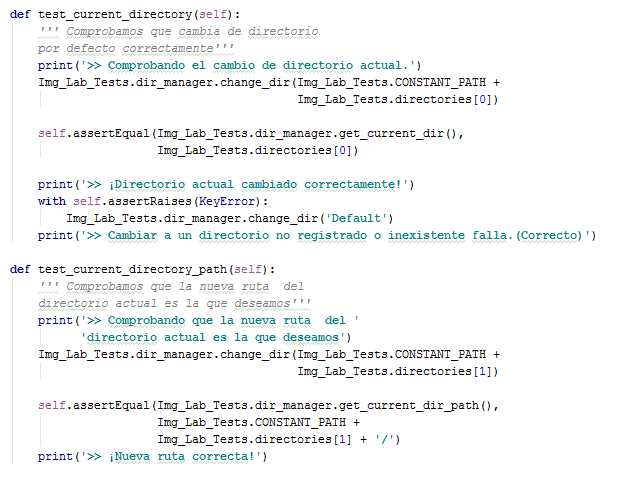
\includegraphics[width=0.99\textwidth]{testex}
\caption{Ejemplo de test unitario}
\label{fig:D.1}
\end{figure}

\begin{figure}
\centering
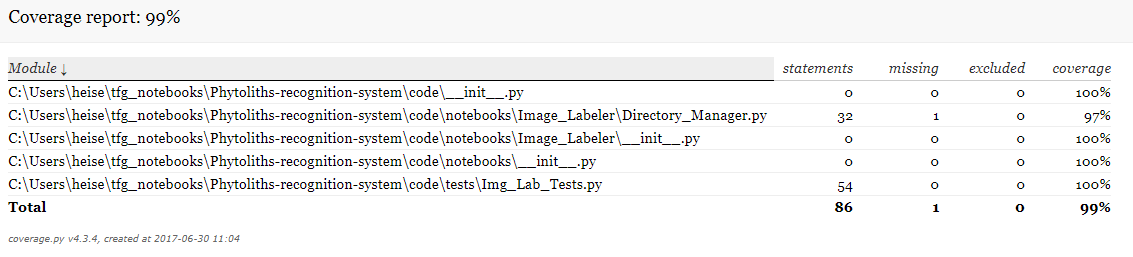
\includegraphics[width=0.99\textwidth]{covex}
\caption{Ejemplo de test unitario}
\label{fig:D.2}
\end{figure}